\section{Results}\label{sec:results}

The study ran \cellsTotal{} cells of \repsPerCell{} replicates each with 200 test points per replicate.
Table~\ref{tab:main} gives the root mean squared error (RMSE) of the main predictors on seven cells that carry the findings
of this section, each with the half-width of its 95\pct{} Monte Carlo interval; the subsections below read the whole grid.

\begin{table*}[!t]
\caption{Root mean squared error, with the half-width of the 95\pct{} Monte Carlo interval, of five predictors on seven cells
of the closed-form study: power (kW) on V0 and V1, throughput (t/h) on V2 and on the capacity study with the engine of the form of
Rocha et al.; 1,900 replicates of 200 test points each. Lower is better.}
\label{tab:main}
\centering\footnotesize
\begin{tabular}{@{}lrrrrr@{}}
\toprule
Cell & Cal. (true) & Cal. KO & LS (c, f80) & Line (c) & Engine refit \\
\midrule
V0, real, n = 10 & 43.8 $\pm$ 0.2 & 46.2 $\pm$ 0.3 & 44.8 $\pm$ 0.2 & 43.5 $\pm$ 0.2 & 67.9 $\pm$ 0.2 \\
V0, surveys, n = 160 & 39.2 $\pm$ 0.1 & 39.4 $\pm$ 0.1 & 39.5 $\pm$ 0.1 & 40.6 $\pm$ 0.1 & 55.4 $\pm$ 0.1 \\
V1($-1$), surveys, 160 & 40.2 $\pm$ 0.1 & 39.8 $\pm$ 0.1 & 39.4 $\pm$ 0.1 & 40.6 $\pm$ 0.1 & 54.5 $\pm$ 0.1 \\
V1(2), surveys, 160 & 39.5 $\pm$ 0.1 & 39.6 $\pm$ 0.1 & 40.2 $\pm$ 0.1 & 41.4 $\pm$ 0.1 & 56.2 $\pm$ 0.1 \\
V2 tph, real, 10 & 164.3 $\pm$ 0.8 & 165.4 $\pm$ 0.8 & 168.5 $\pm$ 0.9 & 181.1 $\pm$ 0.7 & 186.8 $\pm$ 0.6 \\
V2 tph, extrap., 40 & 169.0 $\pm$ 1.2 & 169.0 $\pm$ 1.2 & 170.6 $\pm$ 1.3 & 185.9 $\pm$ 1.6 & 223.5 $\pm$ 0.5 \\
Rocha engine, extrap., 40 & 166.8 $\pm$ 1.2 & 166.9 $\pm$ 1.2 & 171.3 $\pm$ 1.3 & 186.7 $\pm$ 1.6 & 147.0 $\pm$ 0.4 \\
\bottomrule
\end{tabular}

\end{table*}

\subsection{The theory against the simulation}\label{sec:results-theory}

For the four predictors whose risk Theorem~\ref{thm:risk} gives in closed form (the calibrated predictor with the true and
with the shipped scalars, least squares on $\mathbf Z$ and the setting-only line), every cell compares the simulated mean
squared error with the theoretical one computed on the same designs and test points. Over the \zNum{} comparisons the largest
absolute $z$ score is \zMax; \zOverTwo{} exceed 2, against \zExpectTwo{} expected if every difference were Monte Carlo noise,
and \zOverThree{} exceed 3. Figure~\ref{fig:theory-check} plots the pairs on logarithmic axes, where they lie on the identity
line across three orders of magnitude of the error, from the noise floor of the power to the extrapolated throughput. The
theorem therefore describes the simulated risk to within the Monte Carlo error of 1,900 replicates, for all four virtual
plants, the four designs and the five sizes; hypothesis H1's first clause held. The figure does not test the learned
predictors, whose risk has no closed form; they are compared with the theory through the sign tests of the next
subsections and through the full sampler.

\begin{figure*}[!t]
\centering
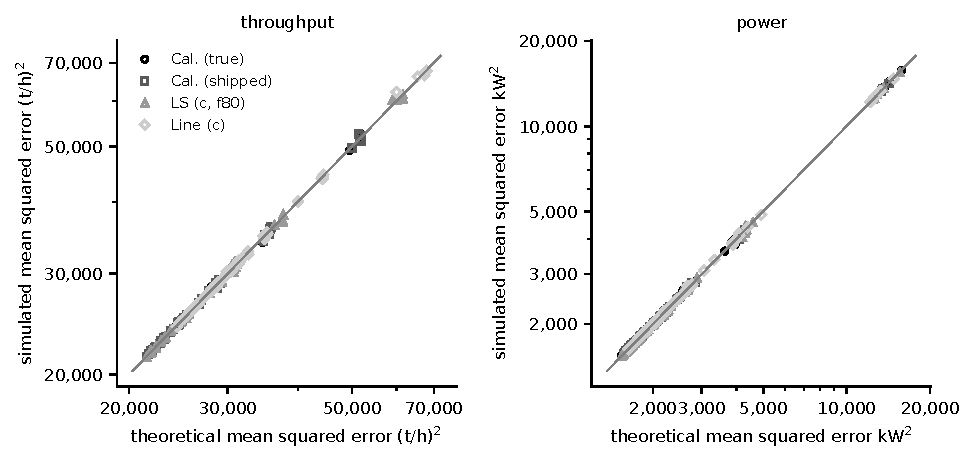
\includegraphics[width=\textwidth]{fig-theory-check}
\caption{Simulated against theoretical mean squared error for the four predictors with a closed-form risk, in every cell of the
study: throughput (left) and power (right). The theoretical value is Theorem~\ref{thm:risk} averaged over each replicate's test
points; the grey line is the identity. The largest of the \zNum{} absolute $z$ scores is \zMax.}
\label{fig:theory-check}
\end{figure*}

\subsection{Curvature alignment}\label{sec:results-align}

The plant V1 puts a share $\alpha$ of the engine's own power curvature into the plant, so Corollary~\ref{cor:align} predicts a
curvature gain $C=(2\alpha-1)\|e_0\|^2$ that changes sign at $\alpha=1/2$. Figure~\ref{fig:align} shows the paired difference of
squared error between the calibrated predictor with the true scalars and least squares, against $\alpha$. With 160 training
surveys the plane gain of Theorem~\ref{thm:fixed} has vanished and the difference is the curvature term alone: on the surveys
window it is $\alAmS$~kW$^2$ at $\alpha=-1$, $\alAhalfS$ at $\alpha=1/2$ and $\alAtwoS$ at $\alpha=2$, against theoretical values
of $-C$ of $-(\alCAmS)$, $-(\alCAhalfS)$ and $-(\alCAtwoS)$. The sign changes exactly at one half, on every design: the engine helps
when the plant carries more than half of the engine's curvature and hurts below. Under extrapolation the same alignment acts
with a larger amplitude ($\alAtwoX$~kW$^2$ at $\alpha=2$), because the test points lie where both curvatures are larger than in
the training window over which the fixed-design term is computed. Adding a curvature that the engine cannot follow,
V1(1, 2), leaves the gain where it was ($\alKqS$~kW$^2$ against $\alAoneS$ without it), as the corollary says: the orthogonal
part of the plant's curvature enters $\mathbf r$ but not $\langle e,r\rangle$.

With ten surveys the picture is different. The plane gain is $\alPlaneTen$~kW$^2$ on the surveys window, three times the
largest curvature gain, and the calibrated predictor beats least squares at every $\alpha$, even at $\alpha=-1$
($\alAmTen$~kW$^2$): with few surveys, what the engine contributes is a shrinkage target for the plane, and its curvature is a
second-order term. The size of the curvature itself bounds what it can ever contribute. The engine's power departs from a
plane in the setting and the feed size by \eRmsS~kW root mean square on the surveys window and \eRmsW~kW on the wide one,
against a noise of \sigKw~kW, so the curvature gain of a perfectly aligned engine ($\alpha=1$) is \curvShareKw\pct{} of the
noise variance. H1 held: the method beats least squares at small shrinkage if and only if the curvature term is positive.

\begin{figure}[!t]
\centering
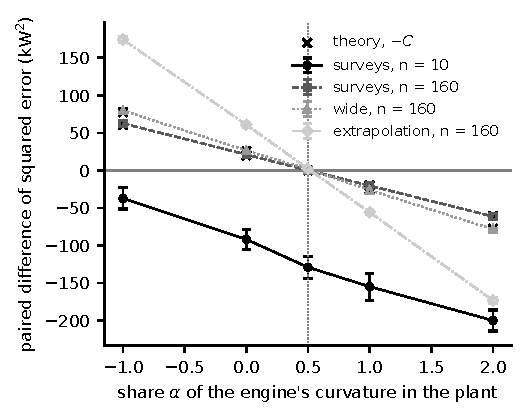
\includegraphics[width=\columnwidth]{fig-align}
\caption{Paired difference of squared error, calibrated predictor with the true scalars minus least squares, on the power of
the plants V1($\alpha$, 0), against the share $\alpha$ of the engine's curvature in the plant (negative: the calibration is
better). Bars: 95\pct{} Monte Carlo intervals over 1,900 replicates. Crosses: $-C$ of Theorem~\ref{thm:fixed} on the training
window. The dotted line marks $\alpha=1/2$.}
\label{fig:align}
\end{figure}

\subsection{Capacity: the affine and the curved forms}\label{sec:results-capacity}

On throughput the shipped engine is affine in the regressors, so by Corollary~\ref{cor:affine} its only contribution is the
shrinkage target. Figure~\ref{fig:capacity} shows the RMSE of the calibrated predictor relative to least squares for the three
engines of the capacity study, on the plant whose capacity is the power law of Rocha et al.~\cite{rocha}. With the affine engine
the ratio is \capAffSTen{} at ten surveys and \capAffSBig{} at 160 on the surveys window, the plane gain decaying as
Theorem~\ref{thm:fixed} predicts; under extrapolation from ten surveys it is \capAffXTen, the largest shrinkage benefit of the
study, and it too vanishes with the surveys (\capAffXBig). With the engine of the plant's own form the ratio stays below one
at 160 surveys: \capRoSBig{} on the surveys window, \capRoWBig{} on the wide one and \capRoXBig{} under extrapolation, a gain that
persists and grows with the width of the window and with the distance of the test points, as H2 stated. Its size is set by the
plant: the plant's capacity departs from a plane by \rRmsTph~t/h root mean square on the surveys window (\rRmsTphW{} on the wide
one) against a noise of \sigTph~t/h, so even an engine of exactly the right form can remove at most \curvCeilTph\pct{} of the
mean squared error.

The engine with half the exponents tests Corollary~\ref{cor:align} where the alignment is not built in. On the surveys window
its curvature is aligned ($\rho=\halfRhoS$) and smaller than the plant's ($\kappa=\halfKappaS$), so it gains
(\capHalfSBig); on the wide window its departure from the plane has another shape ($\rho=\halfRhoW$, $\kappa=\halfKappaW$, so
$\kappa>2\rho$) and it loses (\capHalfWBig), and more under extrapolation (\capHalfXBig). A curvature of the right sign is not
enough: what counts is its projection on the plant's departure from a plane, over the range where predictions are made. The
engine alone, refit without a discrepancy, is the best predictor when its form is exactly the plant's (\capRoRefitXTen{} of
the least-squares RMSE under extrapolation from ten surveys, \capRoRefitSBig{} at 160 on the surveys window) and the worst
when it is not (\capAffRefitSBig{} for the affine engine at 160): the discrepancy is insurance against a wrong form, and it
costs variance when the form is right.

The plant V2 runs the product's engine, with all eight scalars, against the same curved capacity and a power that follows it.
On throughput its result is the affine case: \rVtwoSTenTphOr~t/h for the calibration with the true scalars against
\rVtwoSTenTphLs{} for least squares and \rVtwoSTenTphLine{} for the line at ten surveys, a shrinkage gain only. On power the
engine's curvature is aligned with the plant's but too large ($\rho=\vtwoRho$, $\kappa=\vtwoKappa>2\rho$), the curvature term is
negative ($C=\vtwoC$~kW$^2$), and at 160 surveys the calibration is level with least squares (\rVtwoSBigKwOr{} against
\rVtwoSBigKwLs~kW) while at ten it still gains through the shrinkage (\rVtwoSTenKwOr{} against \rVtwoSTenKwLs). The engine
alone at the scalars of the $L_2$ projection predicts power best at ten surveys (\rVtwoSTenKwEngOr~kW). That projection is a
reference, not a converged optimum: the damped Gauss-Newton iteration reduced the weighted squared distance from \ltwoStart{}
to \ltwoEnd{} in \ltwoIters{} iterations, stopped at its iteration cap with three scalars on the bounds of their priors, and the
oracle predictors of V2 use the scalars where it stopped.

\begin{figure*}[!t]
\centering
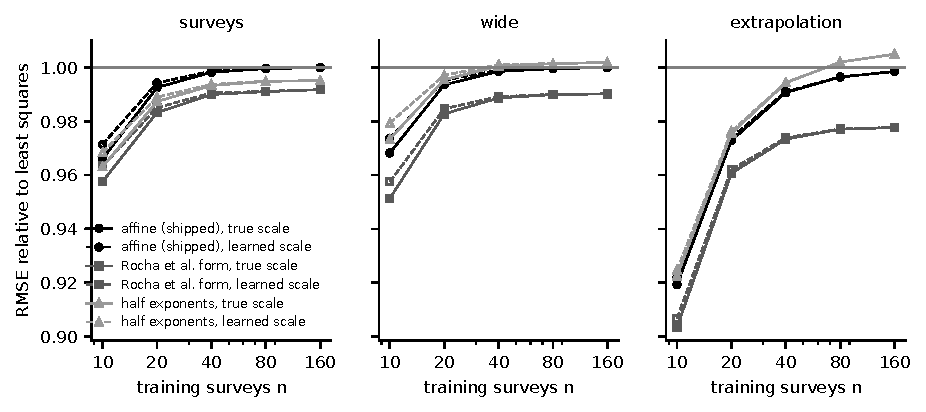
\includegraphics[width=\textwidth]{fig-capacity}
\caption{RMSE of the calibrated throughput predictor relative to least squares on the plant with the capacity law of Rocha et
al., against the number of training surveys, for three engines: the shipped affine capacity, the plant's own power-law form and
the same form with halved exponents; filled markers with the true scale, open markers with the scale learned in the linearized
model. Left to right: surveys window, wide window, extrapolation.}
\label{fig:capacity}
\end{figure*}

\subsection{Sample size, the setting-only line and the discrepancy scale}\label{sec:results-n}

Figure~\ref{fig:nsweep} shows the RMSE on V0 against the number of surveys. On throughput the feed size carries a large
signal beyond the setting ($\phi^2=\phiTwoTphS$~(t/h)$^2$ on the surveys window), so the crossing size of
Proposition~\ref{prop:line} is $n^\star=\nStarTphS$ and every regression on both regressors beats the line from ten surveys on
($\rVzeroSTenTphOr$ against $\rVzeroSTenTphLine$~t/h at $n=10$). On power the feed signal is small ($\phi^2=\phiTwoKwS$~kW$^2$),
the curvature gain is $C=\cFixKwS$~kW$^2$ and $n^\star=\nStarKwS$. The paired difference against the line is
$\lineOrTen$~kW$^2$ at ten surveys, a tie, then $\lineOrTwenty$ at twenty and $\lineOrForty$ at forty, for the predictor with
the true scalars. With the scalars learned the crossing moves later: $\lineKoTen$ at ten, $\lineKoTwenty$ at twenty, a tie, and
$\lineKoForty$ at forty. On the wide window the plane term of~\eqref{eq:line} is positive at ten surveys
($\planeTenKwW$~kW$^2$: the shrinkage pulls toward an engine plane far from the plant's) and the line wins
($\rVzeroWTenKwLine$ against $\rVzeroWTenKwOr$~kW), although $n^\star=\nStarKwW$; the proposition accounts for this through its
plane term, which the crossing size alone omits. H3 held with that qualification: the crossing size locates the overtaking
when the plane term is small, and the full expression~\eqref{eq:line} locates it in every cell. On the real design of the ten
surveys the line is the best predictor of the plant fitted to them ($\rVzeroRealKwLine$~kW against $\rVzeroRealKwOr$ for the
calibration with the true scalars and $\rVzeroRealKwKo$ with learned ones), which is what the held-out comparison
of~\cite{cb002} found on the real surveys.

\begin{figure*}[!t]
\centering
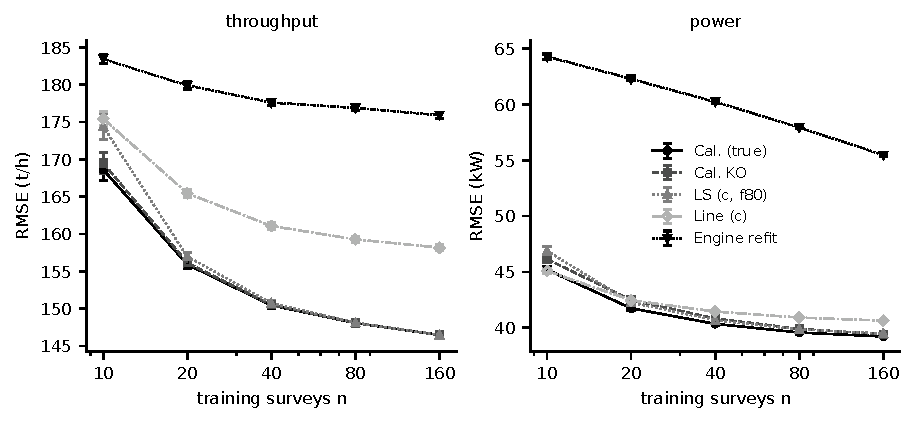
\includegraphics[width=\textwidth]{fig-nsweep}
\caption{RMSE against the number of training surveys on the plant V0 (the engine at the scalars fitted to the ten surveys plus
their fitted discrepancy) over the surveys window, for the calibrated predictor with the true and with the learned scalars,
least squares on the setting and the feed size, the line in the setting and the engine refit without a discrepancy; bars are
95\pct{} Monte Carlo intervals. Left: throughput; right: power.}
\label{fig:nsweep}
\end{figure*}

The discrepancy scale enters through $\lambda=\sigma^2/\tau^2$. Figure~\ref{fig:tau} gives the RMSE of the power prediction with
the true scalars against $\tau$, computed from Theorem~\ref{thm:risk} over 400 designs per size. The risk-optimal scale is
\tauBestTen~kW at ten surveys and \tauBestOneSixty~kW at 160, against the product's 36~kW, and the per-direction optima
of~\eqref{eq:taustar}, the mismatches $|\tilde\delta_k|$ of the engine's and the plant's planes, are \deltaOne, \deltaTwo{} and
\deltaThree~kW. The product's scale sits close to the largest of them and the curve is flat around its minimum:
\tauRmseProdTen~kW at 36 against \tauRmseBestTen~kW at the optimum, for ten surveys. The scale of the discrepancy prior is
therefore not what keeps the method from beating the line on ten surveys ($\tauRmseLineTen$~kW); the noise is.

\begin{figure}[!t]
\centering
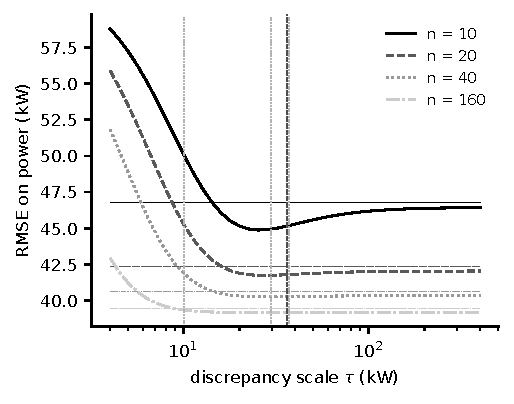
\includegraphics[width=\columnwidth]{fig-tau}
\caption{RMSE on the power of V0 of the calibrated predictor with the true scalars against the discrepancy scale $\tau$, for
four numbers of surveys (thick lines), with least squares at the same sizes (thin lines); dashed: the product's $\tau=36$~kW;
dotted: the plane mismatches $|\tilde\delta_k|$ of~\eqref{eq:taustar}. From Theorem~\ref{thm:risk} over 400 designs per size.}
\label{fig:tau}
\end{figure}

\subsection{The bands}\label{sec:results-bands}

Excluding one plant discussed below, the 80\pct{} band of the calibrated predictor with the true scalars covers between
\covOrMin{} and \covOrMax{} of the test points, with the learned scalars between \covKoMin{} and \covKoMax, and the Student-$t$
band of least squares between \covLsMin{} and \covLsMax. The exact coverage of Corollary~\ref{cor:coverage}, computed on the
plants V0 and V1 over 400 designs, lies between \covExactMin{} and \covExactMax, beside simulated values such as
\covOrSimRealKw{} on the real design and \covOrSimWTenKw{} on the wide window at ten surveys. The coverage falls below nominal
where the theorem places a bias, on the wide window and under extrapolation at small $n$, and the calibrated band stays narrower
than the least-squares band in every cell of Table~\ref{tab:main}. The engine refit without a discrepancy covers as little as
\covRefitMin{} of the test points (its band ignores its own model error), and the calibration at the shipped scalars covers
\covNomMin{} to \covNomMax. The exception is V1(1, 2) under extrapolation: the added curvature grows quadratically outside the
training window, and every band fails there (\covKqXOr{} for the calibration with the true scalars and \covKqXLs{} for least
squares at 160 surveys, \covKqXTenOr{} at ten). No predictor in the study can be trusted outside its training window against a
curvature it does not model.

\subsection{What a design identifies}\label{sec:results-design}

The ceiling of Proposition~\ref{prop:bound} is reached on the ten surveys. The throughput's information about $\ln
Q_{\mathrm{ref}}$ is \ceilInfo{} against the ceiling of \ceilBound{} and a prior precision of \ceilPrior; with throughput alone the
ratio of posterior to prior standard deviation could not fall below \ceilTphOnly. The linearized model with both outputs gives
\ceilLinTen{} on the ten surveys and the sampler of~\cite{cb002} measured \ceilMeasTen, while the floor~\eqref{eq:floor} that no
number of surveys at the fixed speed can pass is \ceilFloor: the ten surveys already give \ceilShare\pct{} of the narrowing of the
capacity base that any campaign at this speed could give. The power sensitivities to $\ln Q_{\mathrm{ref}}$, $\ln W_i$ and
$\ln\zeta$ agree to a relative \productRel, the structural product the floor rests on. Figure~\ref{fig:ceiling} shows the
saturation: \ceilSweepMax{} at \ceilSweepN{} surveys at the fixed speed and \ceilSweepVaried{} with the speed varied over 324,
360 and 396~rpm. Varying the speed does not break the ceiling, because the engine's capacity is flat at its optimum speed (the
factor $s e^{1-s}$ is within 0.6\pct{} of one at ten percent either way), so the sensitivity it moves out of the span of the
discrepancy is a fraction of a percent of the throughput.

\begin{figure}[!t]
\centering
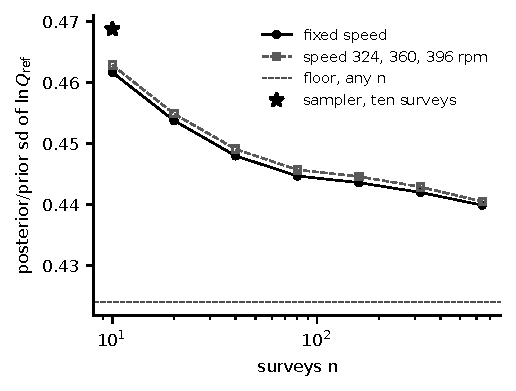
\includegraphics[width=\columnwidth]{fig-ceiling}
\caption{Ratio of posterior to prior standard deviation of the log capacity base against the number of surveys drawn from the
surveys window, in the linearized model with both outputs, at the fixed speed and with the speed varied (mean of 50 designs);
dashed: the floor~\eqref{eq:floor} for any number of surveys at the fixed speed; star: the sampler's value on the ten surveys.}
\label{fig:ceiling}
\end{figure}

Table~\ref{tab:design} and Figure~\ref{fig:design} rank the designs by the expected information gain~\eqref{eq:eig}. The ten
surveys give \eigDzero{} nats. Varying the speed gives \eigDtwo, twenty surveys \eigDthree{} and ten surveys over the wide window
\eigDfour. A measured product size with a noise of 2\pct{} of its mean ($\pEightyMean$~mm) gives \eigPtwo{} nats, more than
doubling the surveys, and at 5\pct{} noise it gives \eigPfive{}, as much as doubling them; at 10\pct{} \eigPten. The product
size is the output that reaches the population-balance scalars: the ratio of $s_{K_1}$ falls from \kOneDzero{} to \kOnePtwo, that
of $s_{K_2}$ to \kTwoPtwo, of $\Delta t_{10}$ to \tTenPtwo{} and of $K_3$ to \kThreePtwo, where throughput and power leave them
near their priors. Twenty surveys also narrow $s_{K_1}$ (\kOneDthree), through the wider spread of settings and feed sizes a
random design has against the ten surveys. H5 held for the product size and failed for the speed: within ten percent of the
capacity optimum, varying the speed teaches nothing that doubling the surveys does not teach better.

\begin{table*}[!t]
\caption{Expected information gain (nats) about the eight scalars and the ratio of posterior to prior standard deviation of
each, in the model linearized at the plant truth with both outputs and their discrepancies, for eight designs; random designs
are the mean of 200 draws. A ratio near one: the design leaves the scalar at its prior.}
\label{tab:design}
\centering\footnotesize
\begin{tabular}{@{}lrrrrrrrrr@{}}
\toprule
Design & EIG (nats) & $Q_{\mathrm{ref}}$ & $W_i$ & $\zeta$ & $P_n$ & $s_{K_1}$ & $s_{K_2}$ & $K_3$ & $\Delta t_{10}$ \\
\midrule
ten surveys (throughput, power) & 1.76 & 0.46 & 0.92 & 0.85 & 0.85 & 0.92 & 0.98 & 0.99 & 0.99 \\
ten surveys, speed 324 to 396 rpm & 1.76 & 0.46 & 0.92 & 0.85 & 0.85 & 0.92 & 0.98 & 0.99 & 0.99 \\
twenty surveys, surveys window & 2.14 & 0.45 & 0.92 & 0.85 & 0.85 & 0.67 & 0.97 & 0.99 & 0.99 \\
ten surveys, wide window & 1.92 & 0.46 & 0.92 & 0.85 & 0.85 & 0.78 & 0.98 & 0.99 & 1.00 \\
ten surveys and P80, noise 10\pct{} & 2.03 & 0.46 & 0.92 & 0.84 & 0.85 & 0.80 & 0.92 & 0.98 & 0.98 \\
ten surveys and P80, noise 5\pct{} & 2.16 & 0.46 & 0.92 & 0.84 & 0.85 & 0.72 & 0.91 & 0.98 & 0.97 \\
ten surveys and P80, noise 2\pct{} & 2.73 & 0.46 & 0.92 & 0.84 & 0.84 & 0.51 & 0.87 & 0.96 & 0.91 \\
P80 (2\pct{}) and varied speed & 2.72 & 0.46 & 0.92 & 0.84 & 0.84 & 0.51 & 0.87 & 0.96 & 0.91 \\
\bottomrule
\end{tabular}

\end{table*}

\begin{figure*}[!t]
\centering
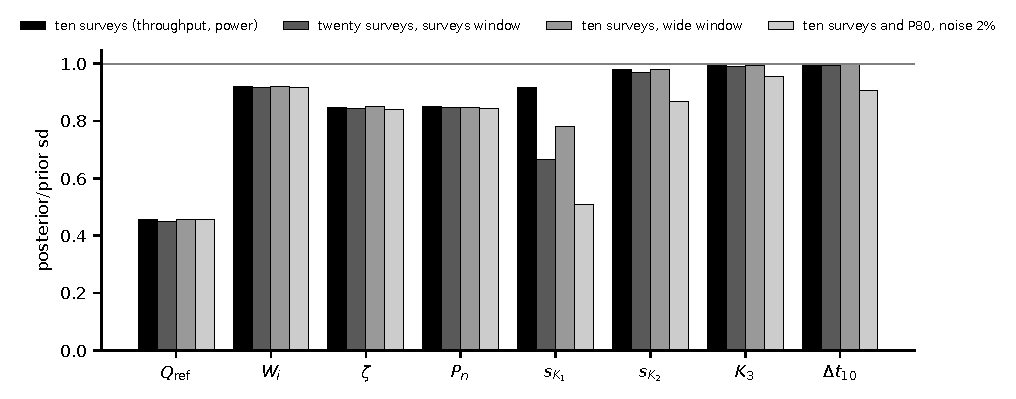
\includegraphics[width=\textwidth]{fig-design}
\caption{Ratio of posterior to prior standard deviation of each of the eight scalars for four designs: the ten surveys, twenty
surveys over the surveys window, ten surveys over the wide window, and the ten surveys with a product-size measurement of 2\pct{}
noise; linearized model at the plant truth. The product size is the only added output that reaches the classification and
breakage scalars.}
\label{fig:design}
\end{figure*}

\subsection{The full sampler}\label{sec:results-sampler}

\sbcText{}

